\newpage

\section{Instalace OpenNebula na RockyLinux 9.5}

\subsection{Základní informace}

Pro tento postup je nutno dodat základní informace zápisu. V příkazových blocích budou značení použití s pravomocemi.

\begin{large}
Značení práv příkazu    
\end{large}

\textbf{\#} administrátorská pravá

\textbf{\$} uživatelské pravá


\subsection{Úvod}

Nutno nainstalovat čistý systém RockyLinux 9.5 v server módu bez žádných balíčků z výběru. Dále budou použity automatizační nástroje pro instalaci ovladačů a základní nastavení. Na \url{https://github.com/KopyTKG/UJEP-LAB} lze najít již předepsané nástroje. 

Pro pokračování budeme předpokládat že systémy Supermicro BMC, BIOS/EUFI a firmware síťové karty byly již aktualizovány na nejnovější možnou verzy.

\newpage

\subsection{Logické zapojení sítě}
Na diagramu lze vidět logické zapojení sítě. Našeb topologie obsahuje 2 oddělené sítě a to jest síť A (192.168.1.0/24) a síť B (10.0.0.0/24). Tyto sítě jsou odděleny z důvodu různých protokolů po kterých komunikují. Síť B je plně izolovaná síť komunikující po InfiniBand\cite{InfiniBand} přesněji přes IPoIB\cite{IPoIB} a síť A používá Ethernet. 

Síť A je použitá jako uplink síť na které se systémy připojují na internet a komunikuje zde IPMI. Síť B je používána jako interní síť pro node to node komunikaci a clustering.


\begin{figure}[!h]
    \centering
    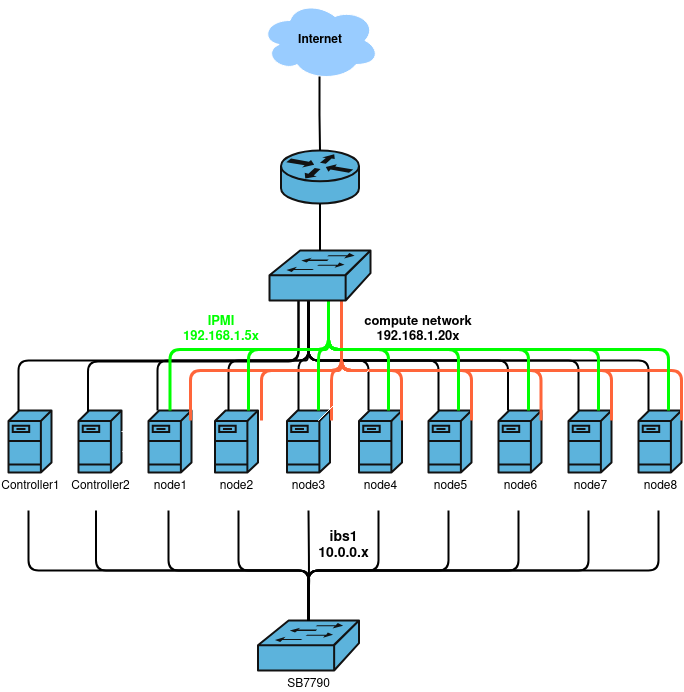
\includegraphics[width=0.8\textwidth]{assets/diagram.png}
    \caption{asd}
    \label{fig:diagram}
\end{figure}


\newpage

\subsection{Poloautomatická instalace}
\label{Skript}
Pro jednoduchost byla sepsána řada skriptů pro automatizování částí instalace celého systému OpenNebula, ovladačů pro InfiniBand\cite{InfiniBand}, MariaDB a Chrony. Jednotlivé kroky těchto skriptů budou vysvětleny v přůběhu návodu.

\begin{small}
\texttt{curl -fsSl https://raw.githubusercontent.com/KopyTKG/UJEP-LAB/refs/heads/Live/\\tools/full.sh | sudo bash}
\end{small}

\subsection{Nastavení síťového připojení}
\label{sitove nastaveni}
Pro jednoduchost nastavení použijeme jíž předinstalovanou aplikaci \textbf{nmcli}. Použití aplikace není nijak složité. V další sekvenci obrázků lze následovat jednoduché kroky pro nastavení interface ibs1 na statickou ip adresu.

Pozor \textit{controller} má jiné pojmenování síťového portu a to jest \textbf{\textit{ibp1s0}}.

\begin{verbatim}
[root@controller]# nmcli con mod ibs1 ipv4.addresses 10.0.0.1/23 ipv4.method manual
[root@controller]# nmcli con mod ibs1 connection.autoconnect yes
[root@controller]# nmcli con up ibs1
\end{verbatim}

\subsection{Nastavení SSH}
Generace klíče není nutná po instalace pomocí skriptu viz \ref{Skript}

Pro plnou funkci je nutno povolit komunikaci pro \textit{root} uživatele. Pro bezpečnost povolíme jen přihlášení pomocí klíče a pro je potřeba vygenerovat klíče přes příkaz \textit{ssh-keygen} s pomocí parametru \textit{-t ed25516}.
\begin{verbatim}
[root@controller]# ssh-keygen -t ed25519 -f /root/.ssh/id_ed25519 -N ""
\end{verbatim}

Z důvodu bezpečnosti nebudeme povolovat přihlášení uživatele root přes heslo a proto je nutno se manuálně přihlásit na každý systém a vytvořit soubor \textit{/root/.ssh/authorized\_keys} s obsahem veřejného klíče z \textit{controller} kde byl vytvořen.

\begin{small}
\texttt{[root@controller]\# cat /root/.ssh/id\_ed25519.pub}\\
\texttt{ssh-ed25519 AAAAC3NzaC1lZDI1NTE5AAAAIC3Qw1k8Qn1v8Qw2Zk1Qw2Zk1Qw2Zk1Qw2Zk1Qw2Zk1Qw2Zk1Q\\w2Zk1Qw2Zk1 root@controller}

\texttt{[root@nodeX]\# echo "ssh-ed25519 AAAAC3NzaC1lZDI1NTE5AAAAIC3Qw1k8Qn1v8Qw2Zk1Qw2Zk1Qw2Zk\\1Qw2Zk1Qw2Zk1Qw2Zk1Qw2Zk1Qw2Zk1 root@controller" \textgreater{}\textgreater{} /root/.ssh/authorized\_keys}
\end{small}

\newpage

\subsection{Přednastavení pro instalaci}
Pro možnost instalace s použitím IPoIB je nutno dodat názvy systémů (Hostname) do \textit{/etc/hosts} a to na všechny stroje kde soubor bude vypadat tak to
\begin{verbatim}
[root@controller]# vim /etc/hosts | nano /etc/hosts

127.0.0.1   localhost localhost.localdomain localhost4 localhost4.localdomain4
::1         localhost localhost.localdomain localhost6 localhost6.localdomain6

10.0.1.1  controller

10.0.0.1  node1
10.0.0.2  node2
10.0.0.3  node3
10.0.0.4  node4
10.0.0.5  node5
10.0.0.6  node6
10.0.0.7  node7
10.0.0.8  node8

192.168.1.201  Eth-node1
192.168.1.202  Eth-node2
192.168.1.203  Eth-node3
192.168.1.204  Eth-node4
192.168.1.205  Eth-node5
192.168.1.206  Eth-node6
192.168.1.207  Eth-node7
192.168.1.208  Eth-node8
\end{verbatim}

po nakonfigurování je nutno ověřit síťové spojení a to ze pomoci \textit{hostname} názvů uvedených v \textit{/etc/hosts}. Testu dosáhneme pomocí jednoduchého ping příkazu.

\begin{verbatim}
[user@controller]$ ping Eth-nodeX
\end{verbatim}

\subsection{Instalace Compute systémů}

\subsection{Základní instalace}

\subsubsection{Instalace NTP serveru}
Jako první krok musím zkontrolovat instalaci a konfigurace NTP serveru. Pro náš testovací cluster byly zvoleny NTS servery od CESNET\cite{CESNET} a to jest \textit{tik.cesnet.cz} a \textit{tak.cesnet.cz}. Pro kontrolu instalace stačí spustit instalaci pomocí příkazu.

\begin{verbatim}
$ sudo dnf install -y chrony
\end{verbatim}

\newpage

Po instalaci použijeme program \textit{tee} pro rychlé přepsáný konfigurace chrony. Tee přepíše celý soubor na následující konfiguraci.

\begin{verbatim}
$ tee /etc/chrony.conf > /dev/null <<EOF
server tik.cesnet.cz iburst
server tak.cesnet.cz iburst

sourcedir /run/chrony-dhcp
driftfile /var/lib/chrony/drift
makestep 1.0 3
rtcsync
keyfile /etc/chrony.keys
ntsdumpdir /var/lib/chrony
leapsectz right/UTC
logdir /var/log/chrony
EOF
\end{verbatim}

Dále jen nutno povolit NTP v firewall a restartovat službu pro znovu načtení konfigurace.
\begin{verbatim}
$ sudo firewall-cmd --permanent --add-service=ntp
$ sudo firewall-cmd --reload
$ sudo systemctl restart chronyd.service
\end{verbatim}

\subsubsection{Instalace SQL databáze}
Pro funk
\begin{verbatim}
$ sudo dnf install mariadb mariadb-server python3-PyMySQL -y
\end{verbatim}

Dále jen nutno přidat konfiguraci

\begin{verbatim}
$ tee /etc/my.cnf.d/openstack.cnf > /dev/null <<EOF
[mysqld]
#nutno pro propojeni IB a Eth (Dashboard a Compute)
bind-address = 0.0.0.0 

default-storage-engine = innodb
innodb_file_per_table = on
max_connections = 4096
collation-server = utf8_general_ci
character-set-server = utf8
EOF
\end{verbatim}

Jako poslední jíž jen spustit službu a dokončit základní konfiguraci

\begin{verbatim}
$ sudo systemctl enable mariadb.service --now
$ sudo mysql_secure_installation
\end{verbatim}

Heslo pro root uživatele (DB\_PASS) si zapište do tabulky viz.: Tabulka hesel \ref{fig:gen-pass-table}

\newpage
\subsubsection{Instalace RabbitMQ}
\subsubsection{Instalace Memcached}

\newpage
\section{Open Nebula}


\begin{figure}[!h]
    \centering
    \begin{tabular}{|l|l|}
    \hline
     \textbf{Název hesla} & \textbf{Heslo} \\
     \hline
     DB\_PASS & 3a81192d09bb454cc35afe06f1cafc5711dec572  \\
     DB\_Oneadmin & 4be5d88f91795e71dce8f4bd626423eef224b30b \\
     KEYSTONE\_DBPASS   & c7246b82ec9b8ca5a7a3fd9f82527e88e2cbc4e6 \\
     GLANCE\_DBPASS     & dca5717ca9bb55581b099e45619da1ffa690e4ce \\
     DASH\_DBPASS       &  \\
     NEUTRON\_DBPASS    & 564b8c564027a33d1cb2e6f724a7a61ca9b9cd0f \\
     NOVA\_DBPASS       & 0eb74ae1f47c0c8495bcf4db9c775a898bc4047b \\
     PLACEMENT\_DBPASS  & d30cfe364a80a7bb53bb758460f325c4292f3f3f \\
     ADMIN\_PASS        & ebf440559b2034e003a4603276ea057cd41ba52e \\
     USER\_PASS         & heslo \\
     GLANCE\_PASS       & 7434063c6875ae43ada80c7267b7437c61ab3845 \\
     DASH\_PASS         &  \\
     NEUTRON\_PASS      & 5b784b0a051a48b23edbd37ac8df53b00819d257 \\
     NOVA\_PASS         & 170b9b7265e0785412ac20cb2539bfde8e21f9bf \\
     PLACEMENT\_PASS    & b54867e5a60c03f0596bdf81f2226886af22e2d7 \\
     \hline
    \end{tabular}
    \label{fig:gen-pass-table}
\end{figure}

CREATE USER 'oneadmin' IDENTIFIED BY '4be5d88f91795e71dce8f4bd626423eef224b30b';
GRANT ALL PRIVILEGES ON opennebula.* TO 'oneadmin';
SET GLOBAL TRANSACTION ISOLATION LEVEL READ COMMITTED;



\begin{verbatim}
repo=$(yum repolist --disabled | grep -i -e powertools -e crb | awk '{print $1}' | head -1)
yum config-manager --set-enabled $repo && yum makecache
 cat << "EOT" > /etc/yum.repos.d/opennebula.repo
[opennebula]
name=OpenNebula Community Edition
baseurl=https://downloads.opennebula.io/repo/6.10/RedHat/$releasever/$basearch
enabled=1
gpgkey=https://downloads.opennebula.io/repo/repo2.key
gpgcheck=1
repo_gpgcheck=1
EOT

yum makecache

dnf install mariadb mariadb-server -y
systemctl enable mariadb.service --now
mysql_secure_installation 
mysql -u root -p
rpm -ivh https://dl.fedoraproject.org/pub/epel/epel-release-latest-9.noarch.rpm
yum -y install opennebula opennebula-fireedge opennebula-gate opennebula-flow opennebula-provision
sudo -u oneadmin /bin/sh
systemctl enable --now  opennebula opennebula-fireedge opennebula-gate opennebula-flow
oneuser show
firewall-cmd --add-port=2616/tcp --permanent
firewall-cmd --reload


\end{verbatim}
\newpage

\subsection{CEPH}

\begin{verbatim}
dnf config-manager --set-enabled crb

dnf install centos-release-ceph-reef -y
dnf install cephadm -y
dnf install ceph-common -y

firewall-cmd --add-port={8443,3000,9095,9093,9094,9100,9283}/tcp --permanent


\end{verbatim}

\subsubsection{Controller}

\begin{verbatim}
cephadm bootstrap --mon-ip 192.168.1.x # Ethernet port pro pripojeni po siti

ssh-copy-id -f -i /etc/ceph/ceph.pub root@*node1 - node8*

ceph orch host add nodeX 10.0.0.X # X = 1 - 8

ceph orch apply osd --all-available-devices
\end{verbatim}

\ukol{libvirt compute\_driver nova.conf} 
\ukol{ update httpd config for placement api}
\ukol{add nova-compute perms to python core}

\newpage

\subsubsection{V}
